% !TEX root = ../../I4PRJ, Grp3 - Rapport.tex
\subsubsection{Implementering}
Den visuelle Implementering af websitet med ASP.NET MVC er skrevet i HTML og CSS. Clientside funktionaliteten er skrevet i JavaScript. Slutteligt er der brugt razor, som er et server-side markup sprog. StatView ses figur~\ref{fig:webstatview}.

\begin{figure}
	\centering
	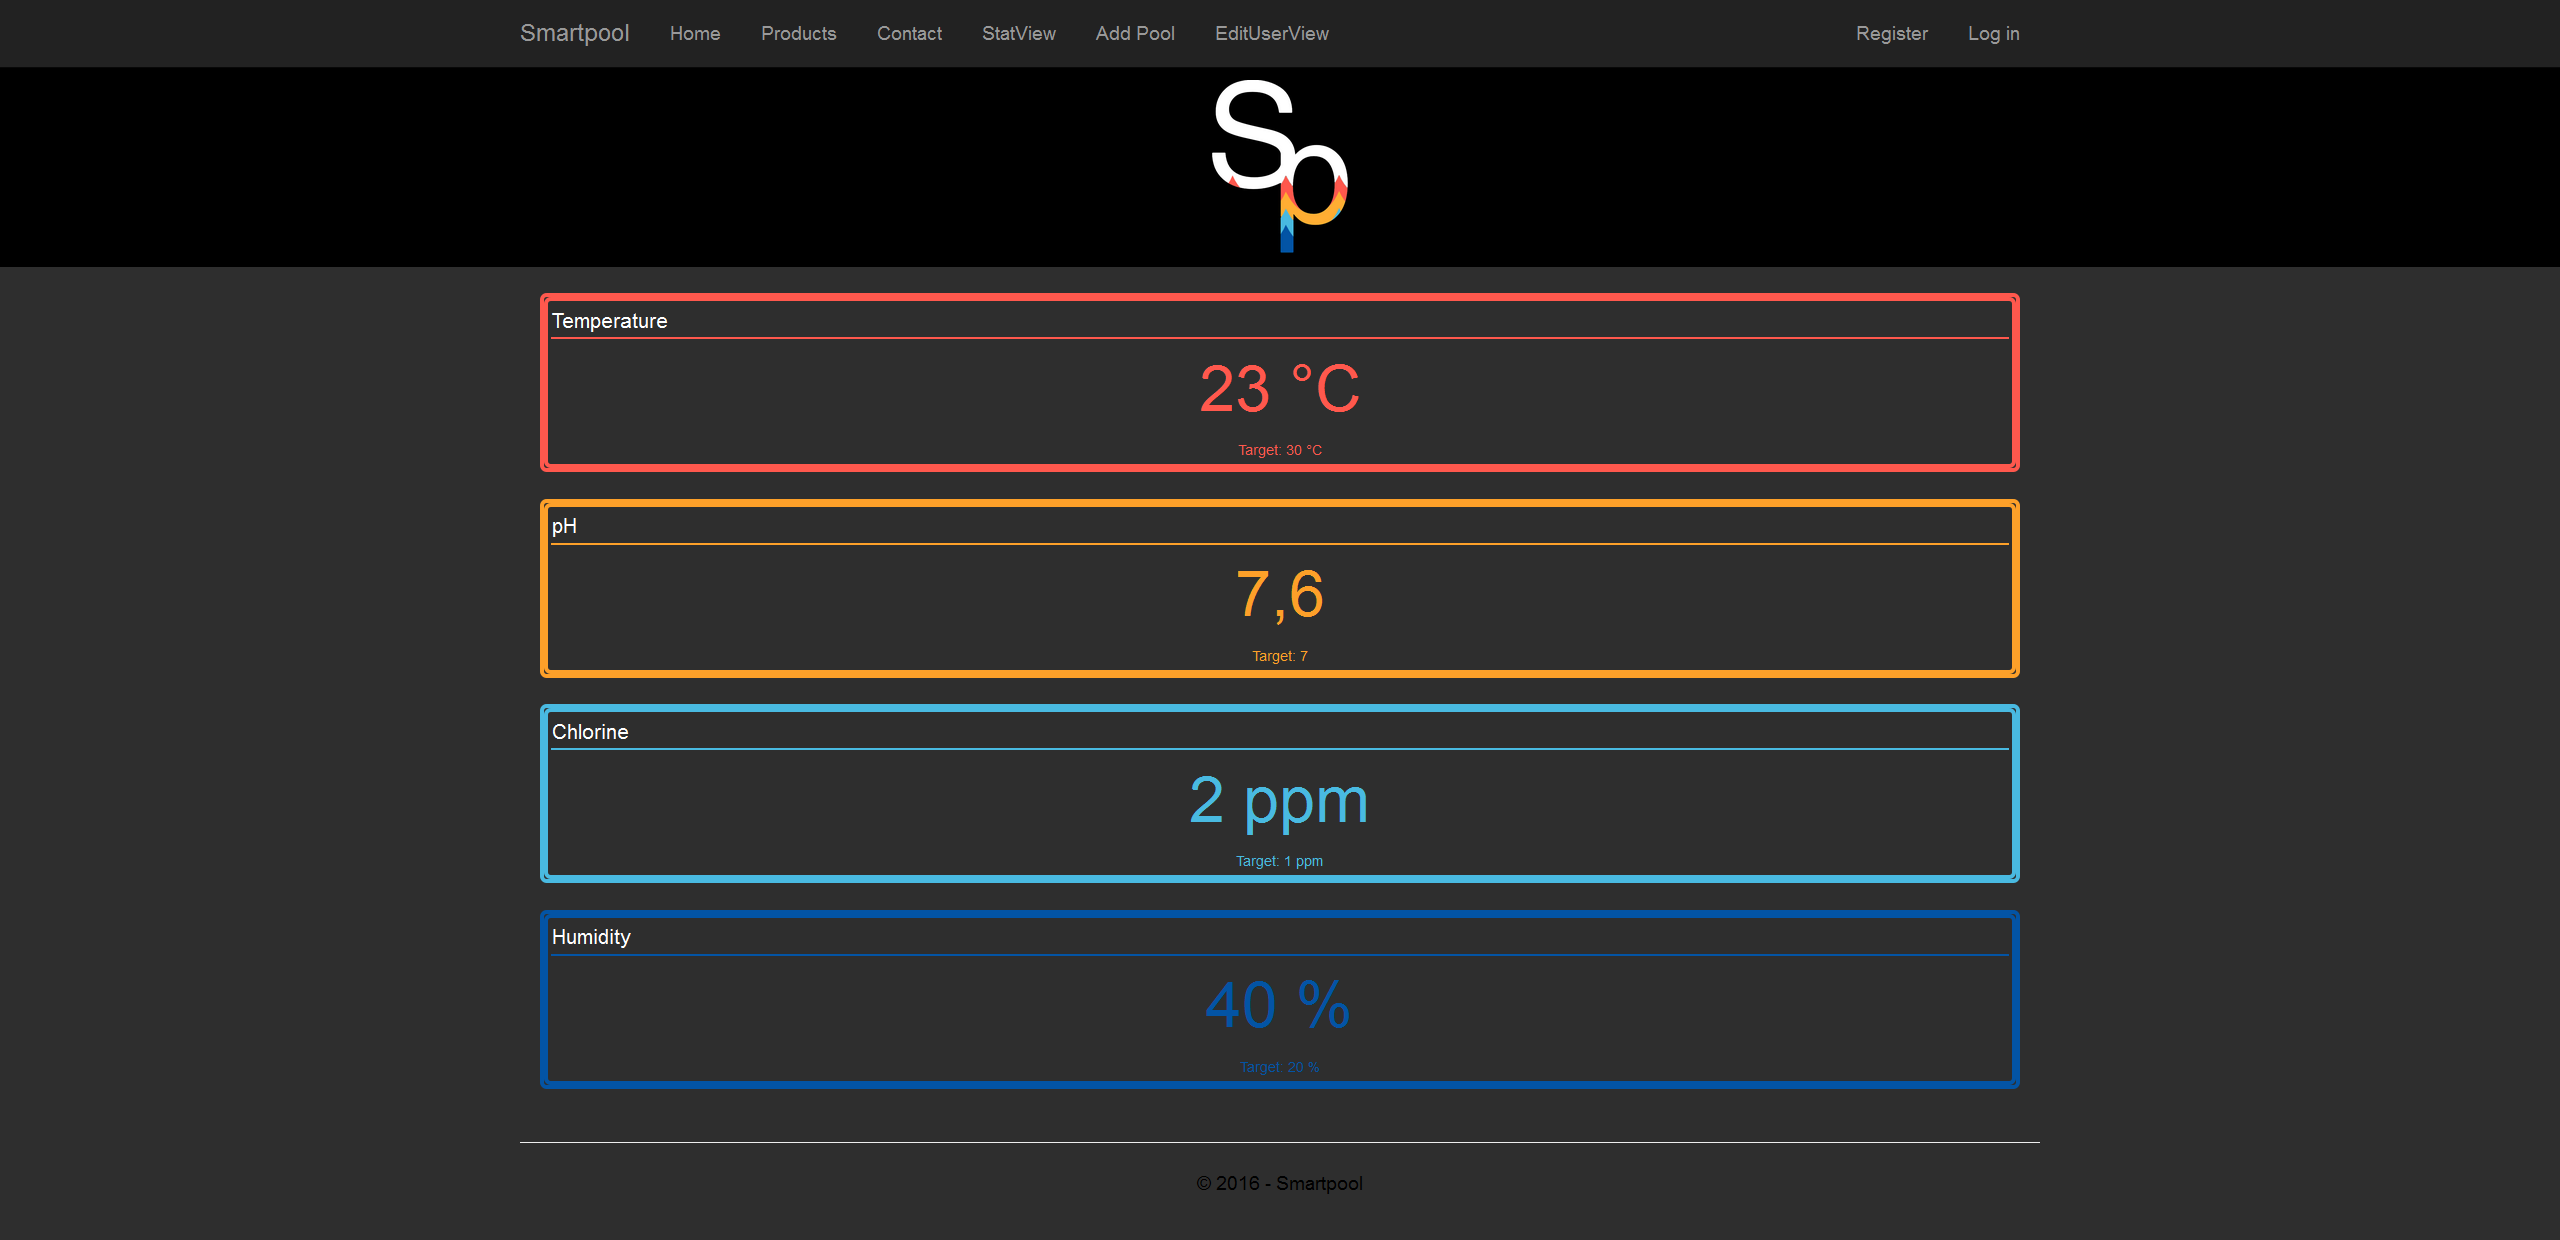
\includegraphics[width=0.9\linewidth]{figs/implementering/web_statview}
	\caption{Web StatView}
	\label{fig:webstatview}
\end{figure}

\paragraph{LoginView}

LoginView ses på figur~\ref{fig:webloginview}.

\begin{figure}
	\centering
	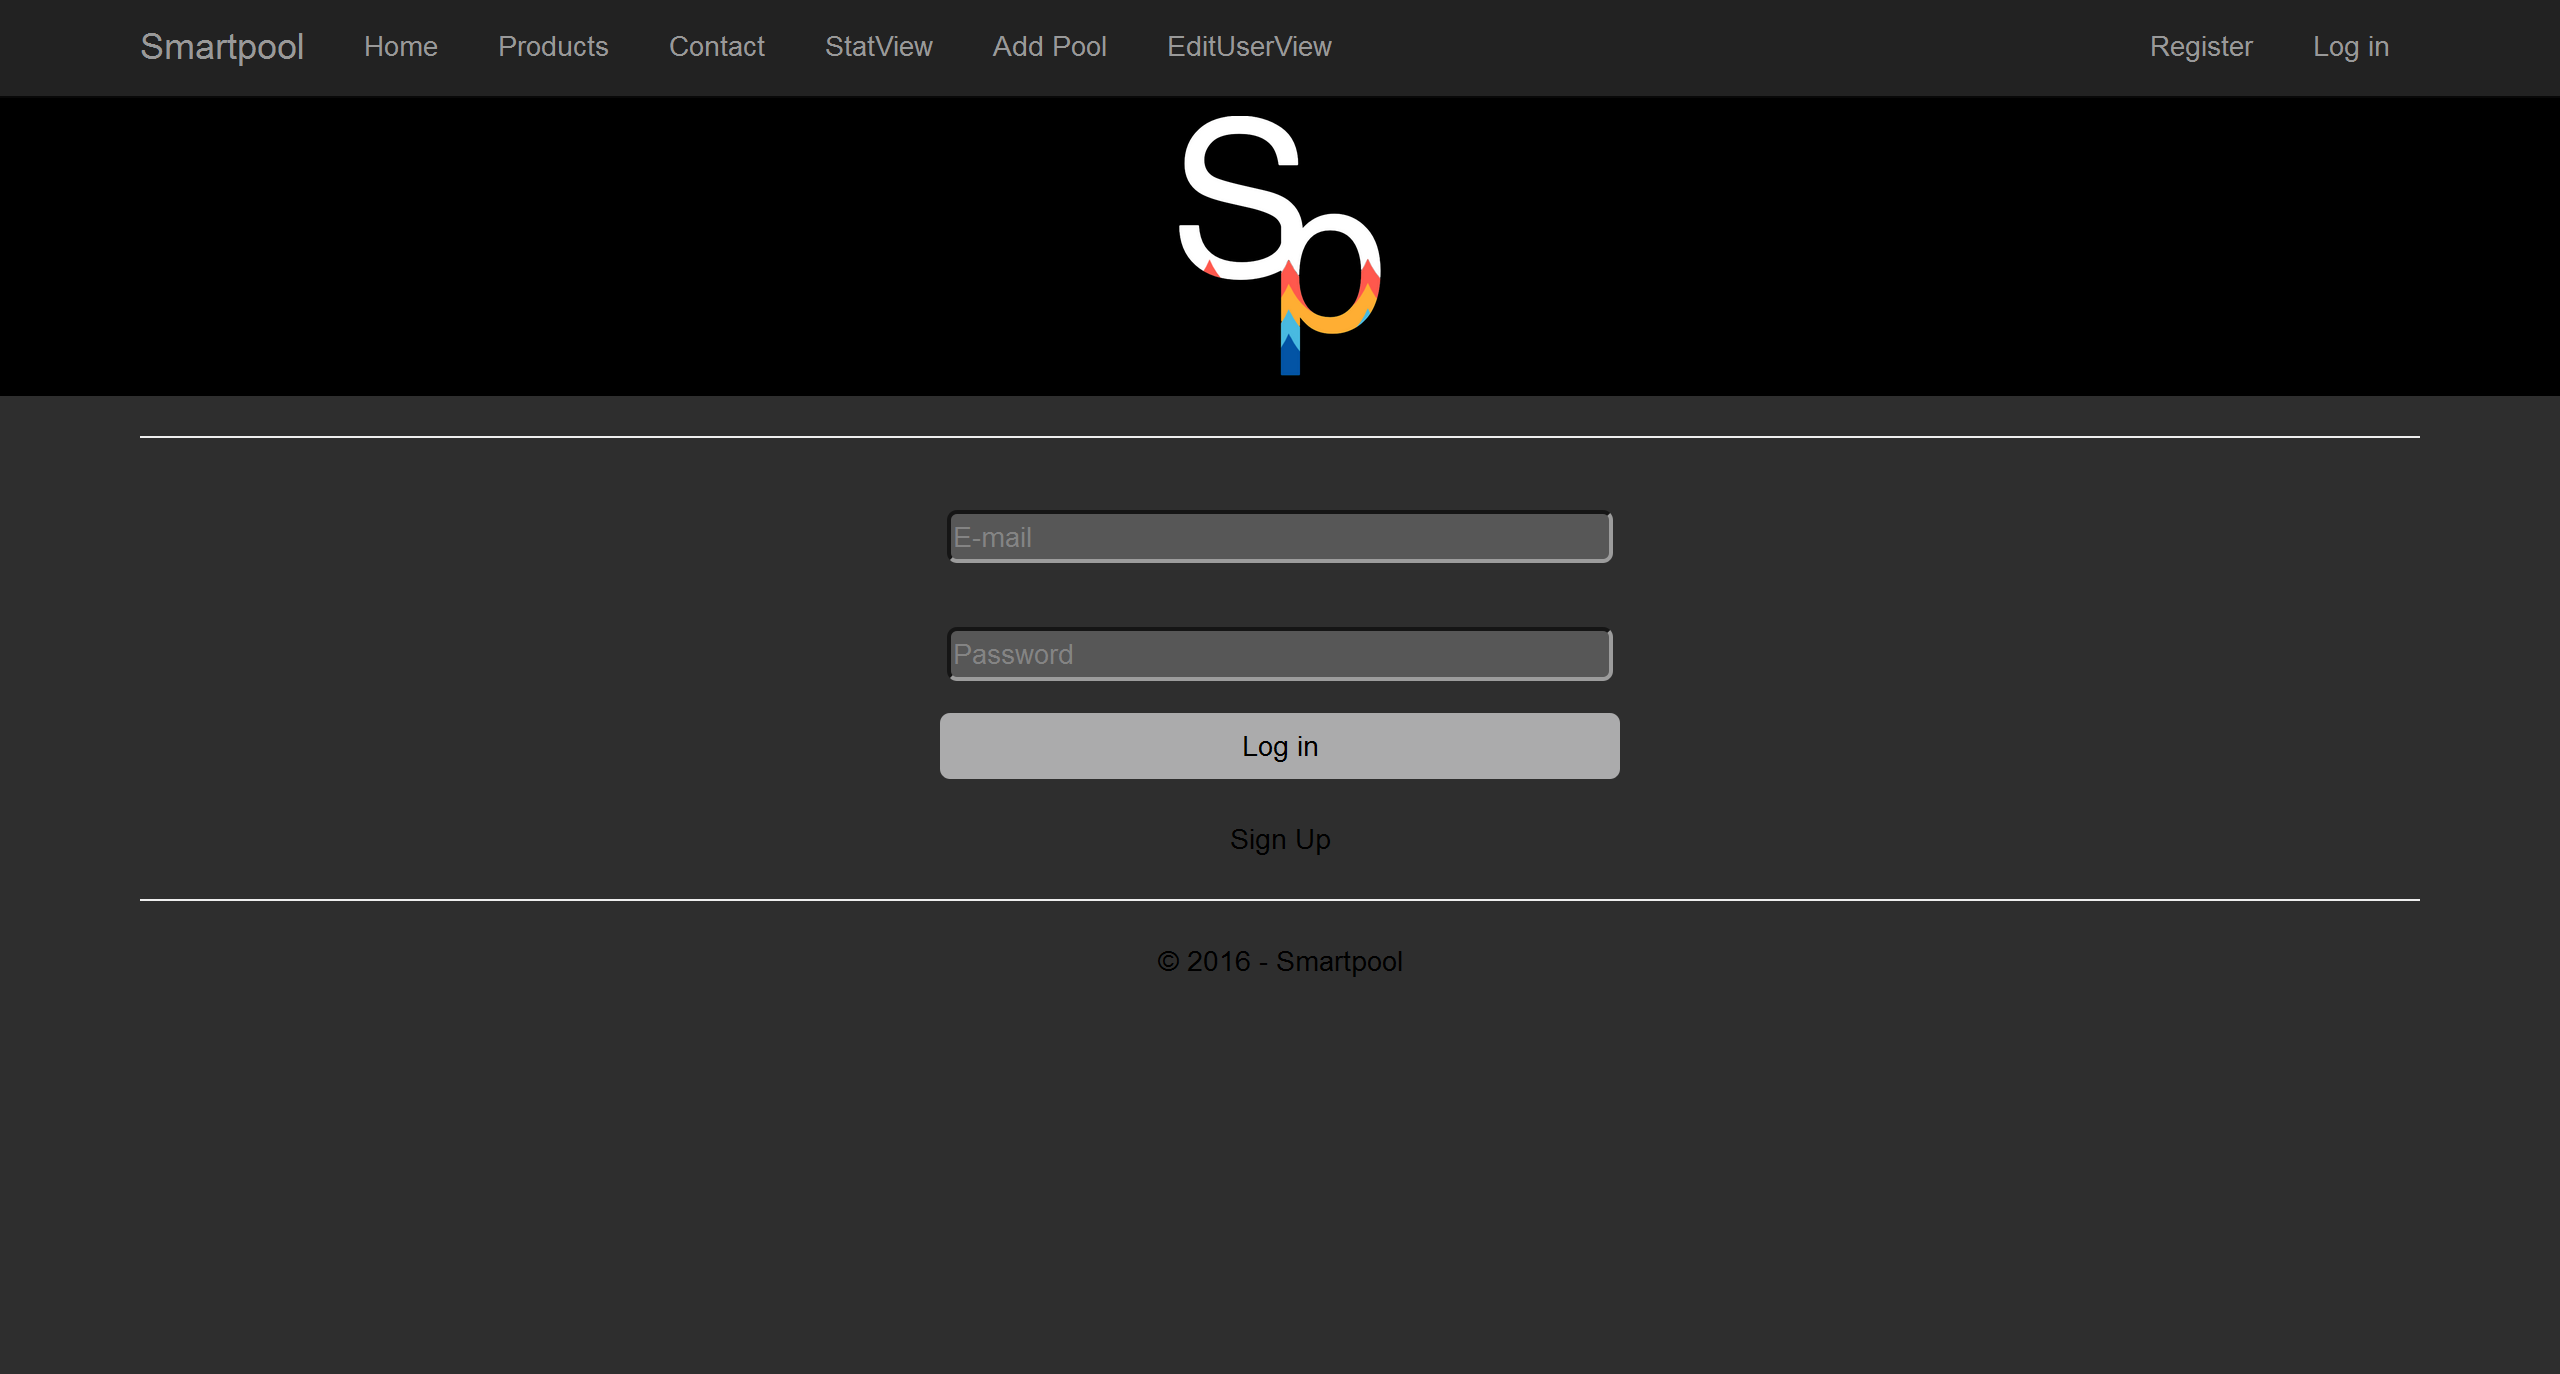
\includegraphics[width=0.9\linewidth]{figs/implementering/web_login}
	\caption{Web LoginView}
	\label{fig:webloginview}
\end{figure}

Når login knappen kalder AccountController, som håndterer login-request, sendes Email og password til presenter. Når svaret på login returneres, kaldes LoginAccepted, som implementeres i AccountController. LoginAccepted vidersender til et andet view på web serveren. For mere information om implementering og kodeeksempel se dokumentationen.

\paragraph{AddPoolView}
AddPoolView ses på figur~\ref{fig:webaddpoolview}:

\begin{figure}
	\centering
	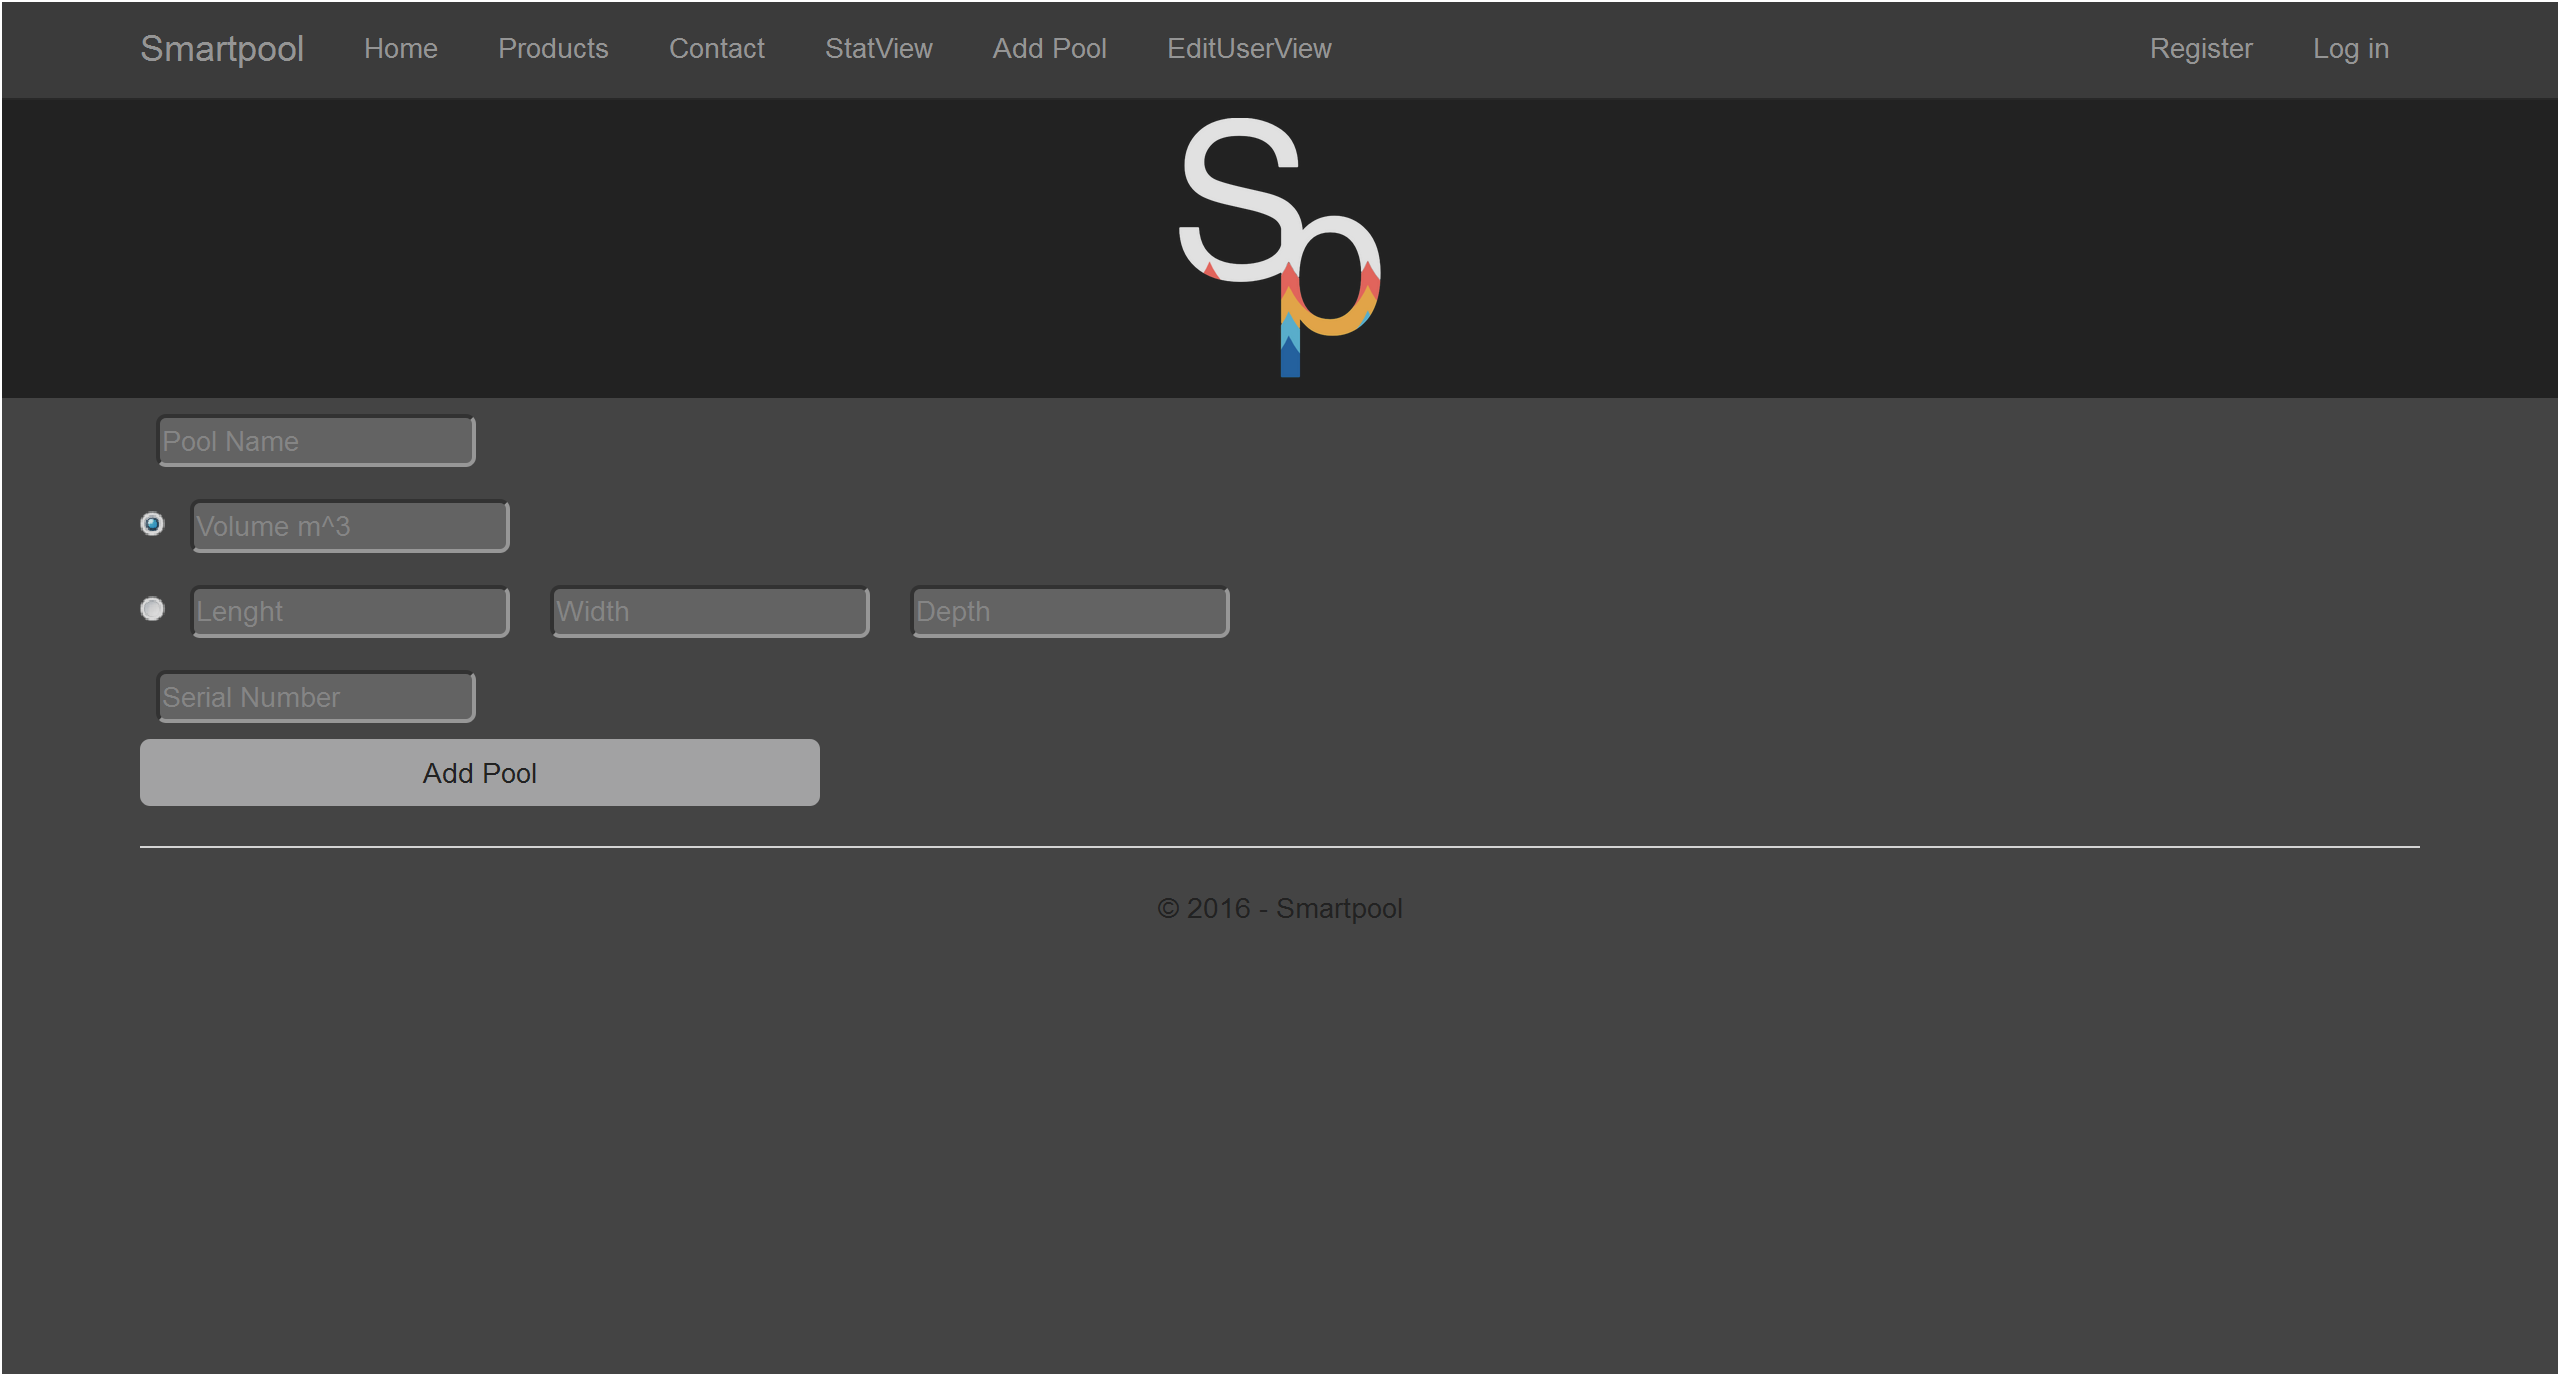
\includegraphics[width=0.9\linewidth]{figs/implementering/web_addpoolview}
	\caption{Web AddPoolView}
	\label{fig:webaddpoolview}
\end{figure}

Brugeren kan vælge enten at indtaste volumen eller dimensioner, ved at vælge på radioknapperne. Når den ene er valgt, er den anden mulighed ikke tilgængeligt. Det håndterer scriptet enableTxtBox. 

Er brugeren begyndt at indtaste volumen, men ombestemmer sig, så bilver tekstfeltet tømt. Det håndteres af scriptet clearText. 

Det er ikke muligt for brugeren at indtaste andet end tal. Det håndterer scriptet isNumber. Disse JavaScripts implementeres i viewet. Mere information om implementering og eksempler se dokumentation.